\subsection{Recommended Build Directory Structure}

Via Autoconf and Automake the Trilinos configuration facilities
provide a great deal of flexibility for configuring and building the
existing Trilinos packages.  However, unless a user has prior experience
with Autotools, we recommend the following process to build and
maintain local builds of Trilinos.

To start, we defined two useful terms:
\begin{itemize}
\item Source tree - The directory structure where source files are found.  A source 
tree is obtained by expanding a distribution tar ball, or by checking 
out a copy of the Trilinos repository.  
\item Build tree - The directory structure where object and library files, as well 
as executables are located.  
\end{itemize}
 
\begin{minipage}[c]{\textwidth}

\begin{minipage}[l]{.6\textwidth}

Although it is possible to run \InlineCommand{./configure} from the source tree (in 
the directory where the configure file is located), we recommend 
separate build trees.  The greatest advantage to having a separate 
build tree is that multiple builds of the libraries can be maintained
from the same source tree.  For example, both serial and parallel libraries
can be built.  
This approach also eliminates problems with configuring in a 'dirty'
directory (one that has already been configured in).
\end{minipage}\hfill
\framebox{\begin{minipage}[r]{.35\textwidth}{
{\bf Key Point:}
$\ldots$ we recommend 
separate build trees $\ldots$ multiple builds of the
libraries can be maintained from the same source tree $\ldots$ 
problems with configuring in a 'dirty' directory (are eliminated) $\ldots$
}\end{minipage}}
\end{minipage}

Setting up a build tree is straight-forward.
Figure~\ref{Figure:TrilinosDirectoryStructure} illustrates the
\begin{figure}
\begin{center}
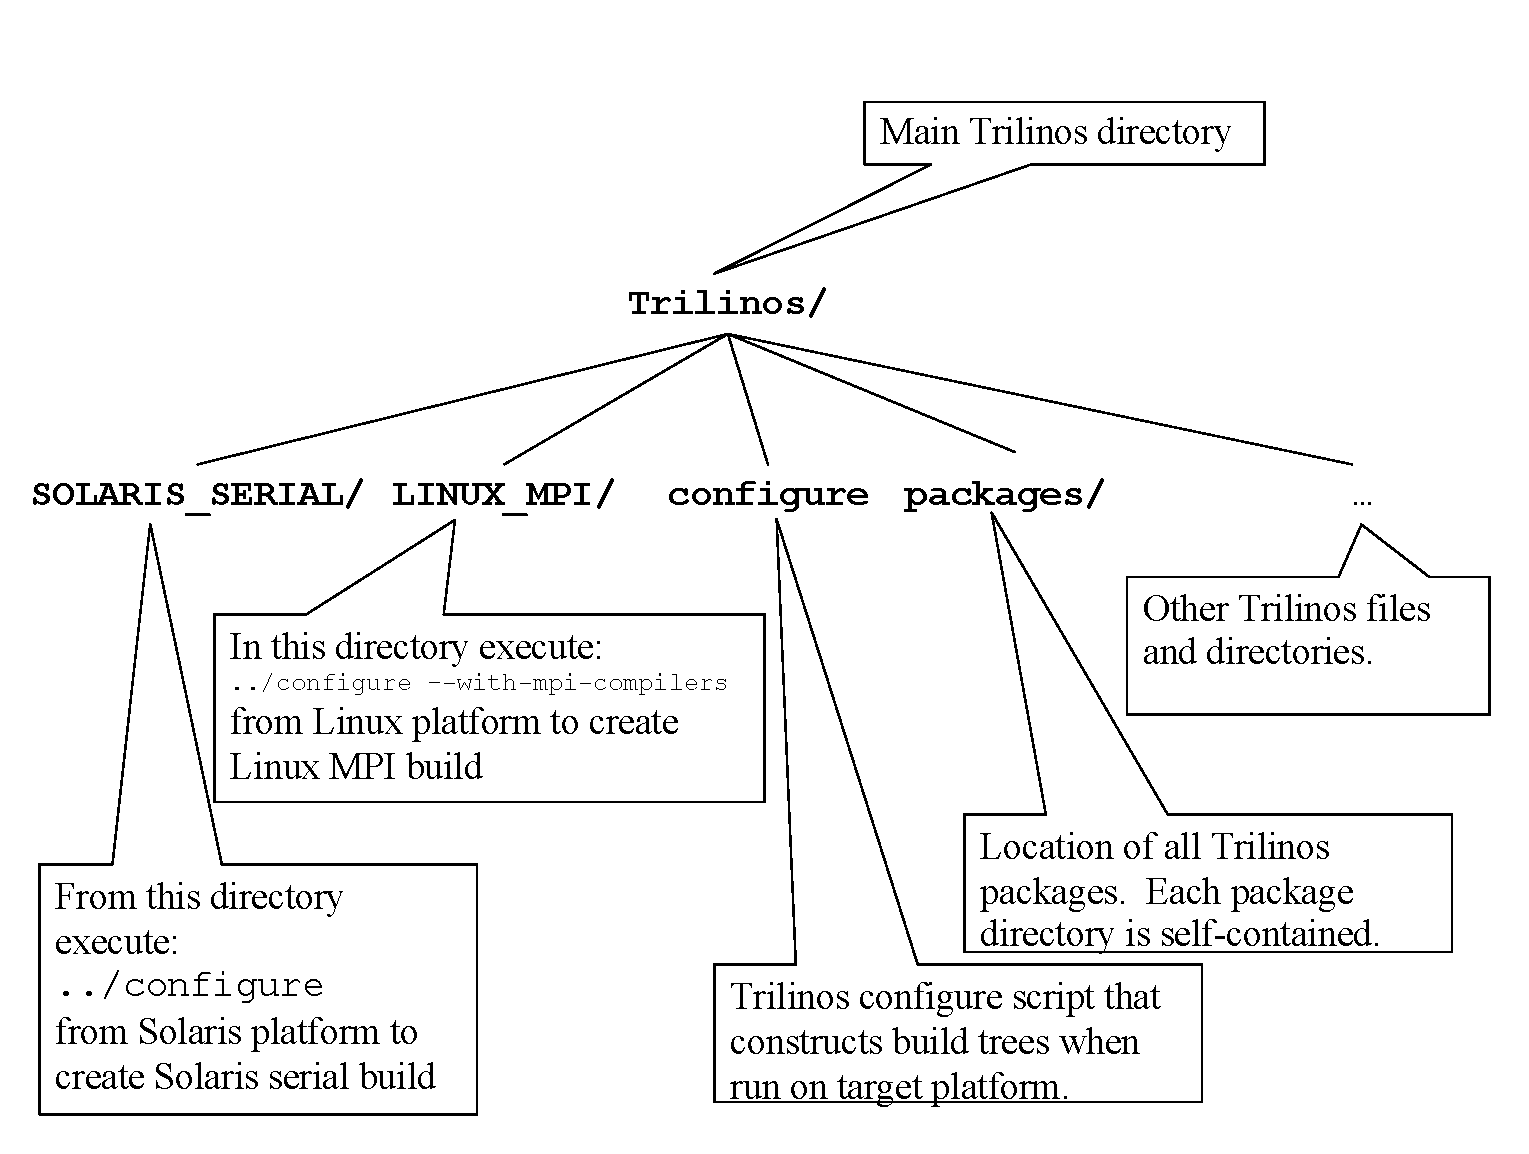
\includegraphics[width=6in]{../CommonFiles/TrilinosDirectoryStructure}
\end{center}
\caption{\label{Figure:TrilinosDirectoryStructure}Recommended Layout for Trilinos Build Directories}
\end{figure}recommended layout.  First, from the highest 
directory in the source tree (Trilinos for a repository copy, Trilinos-3.0.2 
for a distribution), make a new directory - for an MPI build
on a Linux platform, a 
typical name is \InlineDirectory{LINUX\_MPI}.  
Finally, from the new directory, type

\DisplayCommand{../configure --with-mpi-compilers}

(Note that various configure options might be necessary, see Section~\ref{Subsection:ConfiguringTrilinos} for details.)  Finally, type

\DisplayCommand{make}


In summary:

\begin{verbatim}
       cd Trilinos
       mkdir LINUX_MPI
       cd LINUX_MPI
       ../configure --with-mpi-compilers
       make
\end{verbatim}
At this point, the MPI version of Trilinos on a Linux platform is
built and completely contained in the \InlineDirectory{LINUX\_MPI}
directory.  No files outside this directory have been modified.  This
procedure can be repeated for any number of build targets.

{\bf Note:} Although we recommend the above location for build trees,
they can be set up anywhere.

\subsection{Configuring Trilinos}
\label{Subsection:ConfiguringTrilinos}

\begin{minipage}[c]{\textwidth}

\begin{minipage}[l]{.6\textwidth}

The most common issue encountered when configuring Trilinos is that it is 
nearly impossible to determine what caused configure to fail based on the 
standard output.  If the output from configure is inadequate, 
look at the config.log file (in the buildtree)
for the package that failed to configure properly.  

\end{minipage}\hfill
\framebox{\begin{minipage}[r]{.35\textwidth}{
{\bf Key Point:}
$\ldots$ to determine what caused configure to fail $\ldots$ 
look at the config.log file $\ldots$
}\end{minipage}}
\end{minipage}

To determine which 
package failed to configure, look at the bottom of the output from the 
\InlineCommand{configure} command.  One of the last lines will say something 
like:

\begin{verbatim}
    configure: error: /bin/sh '../../../packages/epetra/configure'
    failed for packages/epetra
\end{verbatim}

This particular error indicates to look in 
\InlineDirectory{packages/epetra/config.log}.

	To configure from a remote build tree, simply run the configure script 
in source tree from the root of the build tree.  In the example above, cd to 
the SOLARIS\_SERIAL directory and type 
\DisplayCommand{../configure <configure options>}

A detailed list of configure options can be seen by typing
\DisplayCommand{./configure --help=recursive} from the top level of the 
source tree.  This will display the help page for the Trilinos level as well as all 
Trilinos packages that use Autoconf and Automake.  The output from this command
is quite extensive.  To view the help page for an individual package, cd to 
the home directory for the package in the source tree and type 
\DisplayCommand{./configure --help} 
This command will also display the help page for Trilinos level 
options when used from the Trilinos home directory in the source tree.


Many of the Trilinos configure options are used to describe the details of the 
build.  For 
instance, serial or mpi, all of the packages, or just a proper subset.  

To configure for serial libraries, no action is necessary,
but to configure for parallel libraries, a user must append appropriate 
arguments to the configure invocation line as described in ``Trilinos 
Configuration Options'', section~\ref{subsect:TrilinosConfigOptions}.

Also, to build the default set of Trilinos libraries, no action is 
necessary, but to exclude a package that is built by default, Komplex for 
example, append \newline \InlineCommand{--disable-komplex} to the configure 
invocation  line.  Similarly, to include a package that is not currently built 
by default, NOX for example, append \InlineCommand{--enable-nox} to 
the configure invocation line.  It is recommended that users always configure 
from the Trilinos level and use \InlineCommand{--disable-<package>} as 
necessary, rather than trying to configure from a lower level.  To see which 
packages are built by default and which ones aren't, simply cd to the Trilinos home directory and type \DisplayCommand{./configure --help}


{\bf NOTES:} 
\begin{enumerate}
\item {\bf Ifpack versions:} 
Ifpack is divided into old and new versions.  Future Ifpack developments 
will replace all of Old Ifpack, but at this time some users will need to append
\InlineCommand{--enable-oldifpack} to the configure line.

\item {\bf Enabling/Disabling package builds:} 
The configure process is set up to detect when a 
\InlineCommand{--disable-<package>} option would break a package dependency.  
For example, Ifpack depends on Epetra, so if a user wants to build Ifpack, but 
types \InlineCommand{--disable-epetra}, Epetra will be configured and built 
anyway.  

\item {\bf Installing libraries and header files:}
To install libraries and header files in a particular location, 
use \InlineCommand{--prefix=<dir>} on the configure line.  If this option is 
used, libraries will be located in \InlineDirectory{<dir>/lib} and header files in 
\InlineDirectory{<dir>/include/<package>}.

\item {\bf Providing additional information to Autotools:}
Although Autotools will try to determine all configuration
information, the user must provide anything that Autotools needs and 
cannot find.  Also, if Autotools selects, for example, the wrong 
BLAS library by default, the user must indicate which BLAS library to use.  
Other issues such as standards 
non-compliance are also dealt with here.  If all required libraries (often 
the BLAS and LAPACK) are located in standard places and no special 
compiler flags are required, try configuring without
providing additional information.

\item {\bf Sample configure invocation scripts:}

\begin{minipage}[c]{\textwidth}
\begin{minipage}[l]{.6\textwidth}

Sample configure invocation scripts for a wide variety of platforms can be 
found in \InlineDirectory{Trilinos/config}.  These scripts are 
named using the following convention: \InlineCommand{arch\_comm\_machine}.
For example, \InlineCommand{sgi64\_mpi\_atlantis}.  
\end{minipage}\hfill
\framebox{\begin{minipage}[r]{.35\textwidth}{
{\bf Key Point:}
Sample configure invocation scripts for a wide variety of platforms can be 
found in \InlineDirectory{Trilinos/config}.
}\end{minipage}}
\end{minipage}

Note that these scripts 
are examples only and are primarily useful for the values of options such as 
\InlineCommand{LDFLAGS}, \InlineCommand{CPPFLAGS}, 
and \InlineCommand{CXXFLAGS}.  Do not expect to be able to find a 
script that can be used without modification; try to find a script for a 
similar machine to use as a guide.  

The scripts in the 
repository are not always up to date.  If a user submits a script for a 
machine that few Trilinos developers have an account on, that script may 
become obsolete if it is not updated by the user who submitted it.

Users who create scripts for other machines are encouraged to check them into 
the repository for the benefit of other users.  Users who do not have access to
the repository can send scripts to the Trilinos Library Manager.

The following is an example configure invocation script for an SGI machine:

\begin{verbatim}
../configure --enable-mpi --with-mpi-libs=-lmpi \
--with-cflags=-64 --with-fflags=-64 \
--with-cxxflags="-64 -LANG:std  -LANG:ansi-for-init-scope=ON \
-ptused -DMPI_NO_CPPBIND" \
LDFLAGS=" -64 -L/usr/lib64/mips4/r10000 -L/usr/lib64/mips4 \
-L/usr/lib64 " \
--enable-epetraext --enable-new_package \
--disable-komplex --enable-tsfcoreutils
\end{verbatim}
\end{enumerate}

\subsection{Trilinos Configuration Options}
\label{subsect:TrilinosConfigOptions}
The following options apply to all Trilinos packages unless 
an option doesn't make sense for a particular package (for example, a 
package that does not include any Fortran code will not be sensitive to 
\InlineCommand{F77=g77}), or otherwise noted.  For options specific to 
an individual package, cd to the home directory of the 
package and type \DisplayCommand{./configure --help}.

Basic Options

\begin{itemize}
\item \InlineCommand{--enable-debug} 

(NOX only.)  This turns on compiler debugger flags. It has 
not been fully tested. As an alternate, specify CXXFLAGS on the 
                 configure line.

\item \InlineCommand{--enable-opt}

(NOX only.)  This turns on compiler optimization flags. It 
has not been fully tested. As an alternate, specify CXXFLAGS on the 
                 configure line. 

\item \InlineCommand{--with-cppflags}

Specify additional preprocessor flags (e.g., "-Dflag -Idir") 

\item \InlineCommand{--with-cxxflags}

Specify additional C++ flags 

\item \InlineCommand{--with-ldflags}

Specify additional linker flags (e.g., "-Ldir") 

\item \InlineCommand{--with-ar}

Specify a special archiver command, the default is "ar cru". 
\end{itemize}

 Influential Environmental Variables

\begin{itemize}
\item \InlineCommand{CC}

C compiler command.

\item \InlineCommand{CFLAGS}

C compiler flags.

\item \InlineCommand{CXX}

C++ compiler command.

\item \InlineCommand{CXXFLAGS}

C++ compiler flags.

\item \InlineCommand{LDFLAGS}

Specify linker flags.

\item \InlineCommand{CPPFLAGS}

C/C++ preprocessor flags.

\item \InlineCommand{CXXCPP}

C++ preprocessor.

\item \InlineCommand{F77}

Fortran 77 compiler command.

\item \InlineCommand{FFLAGS}

Fortran 77 compiler flags.
\end{itemize}

MPI-Related Options

\begin{itemize}
\item \InlineCommand{--enable-mpi}

Enables MPI mode. Defines HAVE\_MPI in the (Package)\_Config.h file. Will test 
for the ability to preprocess the MPI header file and may test ability to link 
with MPI.  This option is rarely necessary as many of the below options also 
turn MPI on.  

\item \InlineCommand{--with-mpi-compilers}

Sets CXX = mpicxx (or mpiCC if mpicxx not available), CC = mpicc and 
F77 = mpif77.  Automatically enables MPI mode.  To use compilers other than 
these, specify MPI locations with the below options.  If none of these options 
are necessary, use \InlineCommand{--enable-mpi} to enable MPI mode.  In this 
case, CXX, CC, and F77 have to be set if the correct compilers are 
not chosen by default.

\item \InlineCommand{--with-mpi=MPIROOT}

Specify the MPI root directory. Automatically enables MPI mode.  If this 
option is set, \InlineCommand{--with-mpi-incdir} and 
\InlineCommand{--with-mpi-libdir} should not be used.  
\InlineCommand{--with-mpi} is a shortcut for setting \newline
\InlineCommand{--with-mpi-libdir=MPIROOT/lib} 
and \newline \InlineCommand{--with-mpi-incdir=MPIROOT/include}.

\item \InlineCommand{--with-mpi-libdir=DIR}

Specify the MPI libraries location. Defaults to MPIROOT/lib if 
\InlineCommand{--with-mpi} is specified. If multiple directories must be 
specified, try \newline
\InlineCommand{--with-ldflags="-L<dir1> -L<dir2>"} instead. 

\item \InlineCommand{--with-mpi-libs="LIBS"} 

Specify the MPI libraries. Defaults to \InlineCommand{"-lmpi"}
 if either\InlineCommand{ --with-mpi} or 
\InlineCommand{--with-mpi-libdir} is specified.

\item \InlineCommand{--with-mpi-incdir=DIR}

Specify the MPI include files location. Defaults to \InlineDirectory{MPIROOT/include} if 
\InlineCommand{--with-mpi} is specified. If multiple directories  must be specified, try 
\newline
\InlineCommand{--with-cppflags="-I<dir1> -I<dir2>"} instead.
\end{itemize}

Developer-Related Options
\begin{itemize}
\item \InlineCommand{--enable-maintainer-mode}

Enable make rules and dependencies not useful (and sometimes confusing) to 
the casual installer.
\end{itemize}

\subsection{Building Trilinos}

If the configure stage completed successfully, just type \DisplayCommand{make}
 and then, if 
\InlineCommand{--prefix} was specified, \DisplayCommand{make install}

Other important notes about the configure and build processes.
\begin{itemize}
\item Any code that links to Trilinos should define 
\InlineCommand{HAVE\_CONFIG\_H}.

\item The ``classic'' build system and Autotools do not mix.  Trying to build 
with Autotools in a directory that contains a classic build will not work.  
Before attempting an Autotools build, the classic build object, library, and 
executable files within the source tree should be removed.

\item The build process will fail on OSX if ``DropZip'' is used to 
unzip the Trilinos tarball.  This utility truncates long file names.

\end{itemize}

